\documentclass[pdftex,12pt,a4paper]{article}

\usepackage{graphicx}  
\usepackage[margin=2.5cm]{geometry}
\usepackage{breakcites}
\usepackage{indentfirst}
\usepackage{pgfgantt}
\usepackage{pdflscape}
\usepackage{float}
\usepackage{epsfig}
\usepackage{epstopdf}
\usepackage[cmex10]{amsmath}
\usepackage{stfloats}
\usepackage{multirow}
\usepackage{subcaption} 

\renewcommand{\refname}{REFERENCES}
\linespread{1.3}

\usepackage{mathtools}
%\newcommand{\HRule}{\rule{\linewidth}{0.5mm}}
\thispagestyle{empty}
\begin{document}
\begin{titlepage}
\begin{center}
\textbf{}\\
\textbf{\Large{ISTANBUL TECHNICAL UNIVERSITY}}\\
\vspace{0.5cm}
\textbf{\Large{COMPUTER ENGINEERING DEPARTMENT}}\\
\vspace{2cm}
\textbf{\Large{BLG 242E\\ DIGITAL CIRCUITS LABORATORY\\ EXPERIMENT REPORT}}\\
\vspace{2.8cm}
\begin{table}[ht]
\centering
\Large{
\begin{tabular}{lcl}
\textbf{EXPERIMENT NO}  & : & 5 \\
\textbf{EXPERIMENT DATE}  & : & 15.03.2019 \\
\textbf{LAB SESSION}  & : & FRIDAY - 14.00 \\
\textbf{GROUP NO}  & : & G13 \\
\end{tabular}}
\end{table}
\vspace{1cm}
\textbf{\Large{GROUP MEMBERS:}}\\
\begin{table}[ht]
\centering
\Large{
\begin{tabular}{rcl}
{
150180704  & : & C\.{I}HAT AKK\.{I}RAZ \\
150180707  & : & FAT\.{I}H ALTINPINAR \\
150180734  & : & S\.{I}NAN \c{S}AR \\
}
\end{tabular}}
\end{table}
\vspace{2.8cm}
\textbf{\Large{SPRING 2019}}

\end{center}

\end{titlepage}

\newpage

\thispagestyle{empty}
\centering{\LARGE{ \textbf{ETHIC FORM}}}\\
\centering{\LARGE{\textbf{for}}}\\
\centering{\LARGE{\textbf{BLG242E Logic Circuits Laboratory}}}\\[0.2cm]
As a student of \\Istanbul Technical University Faculty of Computer and Informatics Engineering;
\begin{enumerate}
    \item I will not attempt to cheat in quizes and final exam,
    \item I will not use disallowed sources or tools (mobile phone, calculator etc.) during the exam,
    \item I will not write any information (formula, text, figure etc.) on the table, sheets or books that are allowed to be used during the exam,
    \item I will give reference when using printed or online published sources,
    \item I will not use the results in a source as they are, or by changing a part of them without giving a reference,
    \item I will not show unused sources as used, 
    \item I will not present someone else’s idea as my own idea, 
    \item I will not make someone do my homework, project or thesis for money or anything else,
    \item I will not take an exam or enter a lecture on behalf of others,
    \item I will not make excuses for not attending in exams or lessons by taking reports from someone I know (medical doctor parents or relatives),
    \item I will refrain from deliberately harming the public materials at our university,  
    \item I will comply with the safety rules in laboratory work,
    \item I will behave in accordance with the rules of respect for the lecturers and teaching assistants
\end{enumerate}
\vspace{-1em}
\centering{\LARGE{signed by}}\\
\vspace{-1em}
\begin{table}[ht]
\centering
\begin{tabular}{rcl}
150180704  & : & C\.{I}HAT AKK\.{I}RAZ \\
150180707  & : & FAT\.{I}H ALTINPINAR \\
150180734  & : & S\.{I}NAN \c{S}AR \\
\end{tabular}
\end{table}
\vspace{-1em}
 \begin{table}[ht]
 \begin{tabular}{lr}
%\textbf{Date:\hspace*{1.0cm}/\hspace*{1.0cm}/} &\qquad \qquad\qquad\qquad \qquad\qquad\qquad \qquad\qquad\qquad \qquad\qquad \textbf{SIGNED}\\
\end{tabular}
\end{table} % adds the ethic sign
\addcontentsline{toc}{section}{\numberline {}ETHICS}
\newpage

\thispagestyle{empty}
\addtocontents{toc}{\contentsline {section}{\numberline {}FRONT COVER}{}}
\addtocontents{toc}{\contentsline {section}{\numberline {}CONTENTS}{}}
\setcounter{tocdepth}{4}
\tableofcontents
\clearpage

\setcounter{page}{1}

\section{INTRODUCTION}
\begin{flushleft}
\paragraph{}
In this experiment we have built various circuits in order to observe and understand the differences between TTL and CMOS gate families. 
\end{flushleft}

\section{REQUIREMENTS}
\begin{flushleft}
\underline{Tools Used}\cite{booklet}
\end{flushleft}
\begin{itemize}
    \item C.A.D.E.T
    \item Integrated Circuits
    \begin{itemize}
        \item 74xx00 TTL NAND Gates
        \item 4011 CMOS NAND Gates  
    \end{itemize}
    \item Oscilloscope
    \item 100$\Omega$ Resistor
\end{itemize}

\begin{flushleft}
\subsection{Part 1}
\paragraph{}
In this part of the experiment, every given circuit is built with NAND gates from both CMOS and TTL families. With the aid of the potentiometer, voltage values are changed on the circuit in order to record how NAND gates behave.  
\end{flushleft}


\begin{flushleft}
\subsubsection{Part 1.a}

 \begin{figure}[h]
    	\centering
    	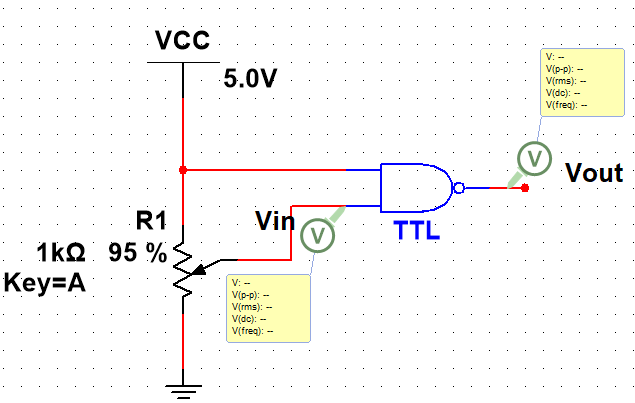
\includegraphics[width=0.5\textwidth]{part1a-ttl.png}	
    	\caption{The circuit using TTL NAND gate.}
    	\label{fig:1-part1a-ttl}
\end{figure}

\paragraph{} % burdayim burdayim hi hi hi hi hi hi hi h ih ih ih ih hi hi hi h i goruyon mu
The circuit given in Figure \ref{fig:1-part1a-ttl} is implemented using a TTL NAND gate. Then with the aid of the potentiometer $V_{input}$ is changed several times in order to observe it's effects on $V_{output}$. All results of the mentioned part are given in Table \ref{part1a-TTL}


%Table of part1a-ttl
\begin{table}[h]

\begin{tabular}{c|c|c|c|c|c|c|c|}
                   & 1    & 2    & 3    & 4    & 5    & 6    & 7    \\ \hline
$V_{input} (Volt)$ & 0.00 & 0.35 & 1.04 & 2.27 & 3.43 & 4.60 & 4.96 \\ \hline
$V_{output}(Volt)$       & 3.71 & 3.86 & 3.52 & 0.19 & 0.20 & 0.20 & 0.26
\end{tabular}
\centering
\caption{Switching Characteristics of TTL}
\label{part1a-TTL}
\end{table}

 \begin{figure}[h]
    	\centering
    	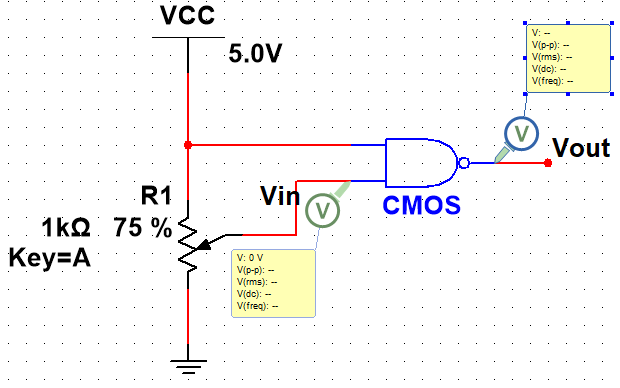
\includegraphics[width=0.5\textwidth]{part1a-cmos.png}	
    	\caption{The circuit using CMOS NAND gate.}
    	\label{fig:2-part1a-cmos}
\end{figure}

\paragraph{}
%Same procedure xd
% seninki gibi yapayım hepsini :) sen başk tamamdır ''^
% mantikli satmayalim en son bakariz boyle kala da bilir ben sonuclari yazmaya caliscam sen bu sekilde hepsine ekle o zmn
The circuit given in Figure \ref{fig:2-part1a-cmos} is implemented using a CMOS NAND gate. Then with the aid of the potentiometer $V_{input}$ is changed several times in order to see it's effects on $V_{output}$. All results of the mentioned part are given in Table \ref{part1a-CMOS}.


%Table of part1a-cmos
\begin{table}[h]
\begin{tabular}{c|c|c|c|c|c|c|c|}
                   & 1    & 2    & 3    & 4    & 5    & 6    & 7    \\ \hline
$V_{input} (Volt)$ & 0.00 & 0.74 & 1.66 & 2.94 & 3.49 & 4.39 & 4.96 \\ \hline
$V_{output}(Volt)$       & 4.95 & 4.95 & 4.95 & 0.13 & 0.15 & 0.25 & 0.16
\end{tabular}
\centering
\caption{Switching characteristics of CMOS}
\label{part1a-CMOS}
\end{table}
\end{flushleft}

\newpage

 \begin{figure}[h]
    	\centering
    	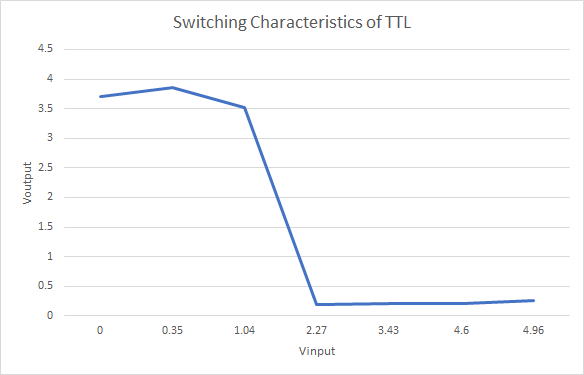
\includegraphics[width=0.7\textwidth]{charts/part1a-chart.png}	
    	\caption{Switching characteristics of TTL}
    	\label{graph:3-part1a-ttl}
\end{figure}

 \begin{figure}[h]
    	\centering
    	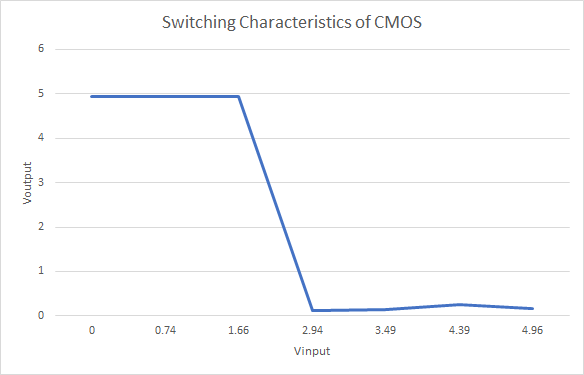
\includegraphics[width=0.7\textwidth]{charts/part1a-cmos-chart.png}	
    	\caption{Switching characteristics of CMOS}
    	\label{graph:3-part1a-cmoss}
\end{figure}


\begin{flushleft}
\paragraph{}
Figure \ref{graph:3-part1a-ttl} and Figure \ref{graph:3-part1a-cmoss} are the graphs of the function $f(V_{output}) = V_{output}$. It is a clear fact that CMOS is much more stable than TTL while producing high output. Both gates does not have state between low and high. Another information that can be extracted from these graphs is TTL's noise margin is greater than CMOS's.  
\end{flushleft}






\newpage
\begin{flushleft}
\subsubsection{Part 1.b}


 \begin{figure}[h]
    	\centering
    	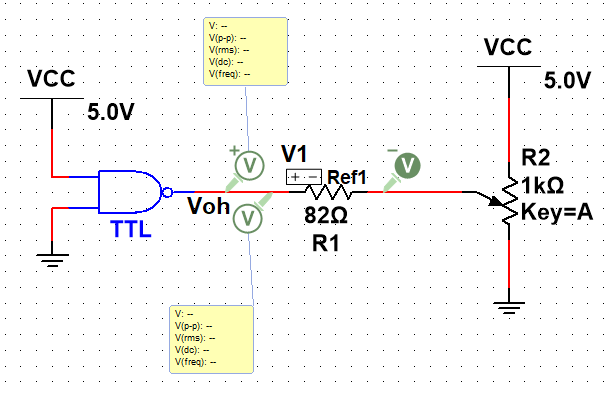
\includegraphics[width=0.5\textwidth]{part1b-ttl.png}	
    	\caption{The circuit using a TTL NAND gate.}
    	\label{fig:3-part1b-ttl}
\end{figure}

\paragraph{}The circuit given in figure \ref{fig:3-part1b-ttl} is implemented using a TTL NAND gate. The aim of this part is to find the maximum possible value of $I_{AB}$ when the output state of the gate is Logic-1. With the aid of the potentiometer $V_{output}$ is changed several times in order to see it's effects on $V_{AB}$. $I_{OH}$ values are calculated by using $V_{OH}/R$. All results are given in Table \ref{part1b-ttl}.

%Table of part1b-ttl
\begin{table}[h]
\begin{tabular}{c|c|c|c|c|c|c|c|}
                & 1    & 2    & 3    & 4    & 5    & 6    & 7    \\ \hline
$V_{AB} (Volt)$ & 2.12 & 1.72 & 1.25 & 0.87 & 0    & 0    & 0    \\ \hline
$V_{OH} (Volt)$ & 2.20 & 2.50 & 2.85 & 3.12 & 3.96 & 4.54 & 4.95 \\ \hline
$I_{OH} (mA)$   & 25.8 & 20.9 & 15.2 & 10.6 & 0    & 0    & 0   
\end{tabular}
\centering
\caption{$V_{OH} - I_{OH}$ Characteristics of TTL}
\label{part1b-ttl}
\end{table}


 \begin{figure}[h]
    	\centering
    	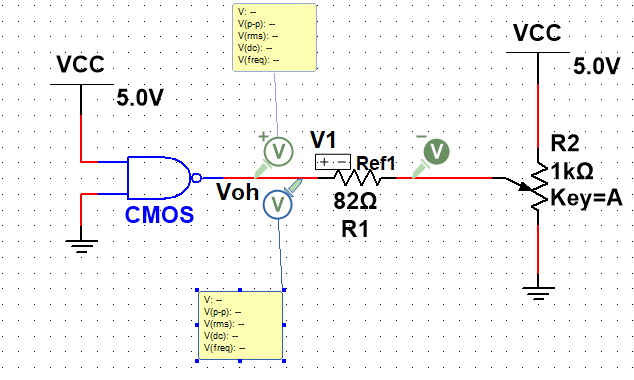
\includegraphics[width=0.5\textwidth]{part1b-cmos.png}	
    	\caption{The circuit using a CMOS NAND gate.}
    	\label{fig:3-part1b-cmos}
\end{figure}

\paragraph{}The circuit given in figure \ref{fig:3-part1b-cmos} is implemented using a CMOS NAND gate. The aim of this part is to find the maximum possible value of $I_{AB}$ when the output state of the gate is Logic-1. With the aid of the potentiometer $V_{output}$ is changed several times in order to see it's effects on $V_{AB}$. $I_{OH}$ values are calculated by using $V_{OH}/R$. All results of the mentioned part are given in Table \ref{part1b-cmos}.



%Table of part1b-cmos
\begin{table}[h]
\begin{tabular}{c|c|c|c|c|c|c|c|}
                & 1    & 2    & 3    & 4    & 5    & 6    & 7    \\ \hline
$V_{AB} (Volt)$ & 0.48 & 0.47 & 0.44 & 0.41 & 0.32 & 0.21 & 0.02 \\ \hline
$V_{OH} (Volt)$ & 0.49 & 1.01 & 1.56 & 2.28 & 3.27 & 3.96 & 4.95 \\ \hline
$I_{OH} (mA)$   & 5.85 & 5.73 & 5.37 & 5.00 & 3.90 & 2.56 & 0.24
\end{tabular}
\centering
\caption{$V_{OH} - I_{OH}$ Characteristics of CMOS}
\label{part1b-cmos}
\end{table}
%kayarsa garip oluyor below above.



\newpage
\paragraph{}
In the figures below(Figure \ref{graph:3-part1b-ttl} and \ref{graph:3-part1b-cmoss}), we can see the switching characteristics for both CMOS and TTL for above mentioned circuits. We were able to observe a wider voltage range with CMOS than we were ablo to with TTL. This can be interpreted as TTL being less reactive to changes in resistance and therefore current in the circuit.
 \begin{figure}[h]
    	\centering
    	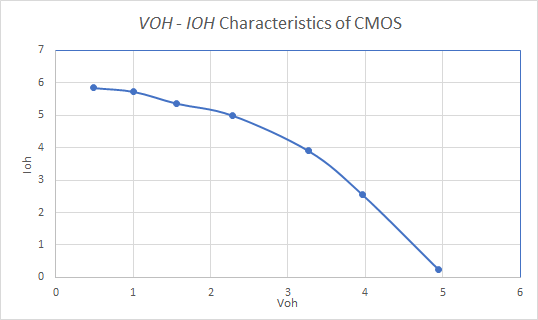
\includegraphics[width=0.7\textwidth]{charts/part1b-cmos-chart.png}	
    	\caption{$V_{OH} - I_{OH}$ Characteristics of TTL}
    	\label{graph:3-part1b-ttl}
\end{figure}

 \begin{figure}[h]
    	\centering
    	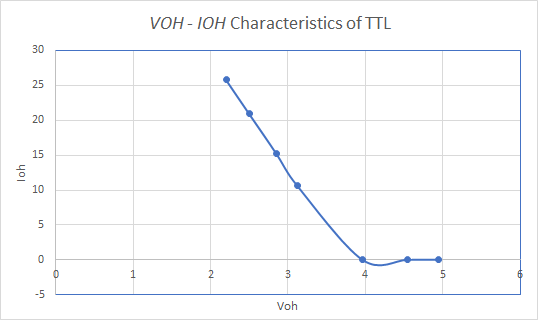
\includegraphics[width=0.7\textwidth]{charts/part1b-ttl-chart.png}
    	\caption{$V_{OH} - I_{OH}$ Characteristics of CMOS}
    	\label{graph:3-part1b-cmoss}
\end{figure}



\end{flushleft}



\newpage
\begin{flushleft}
\subsubsection{Part 1.c}

 \begin{figure}[h]
    	\centering
    	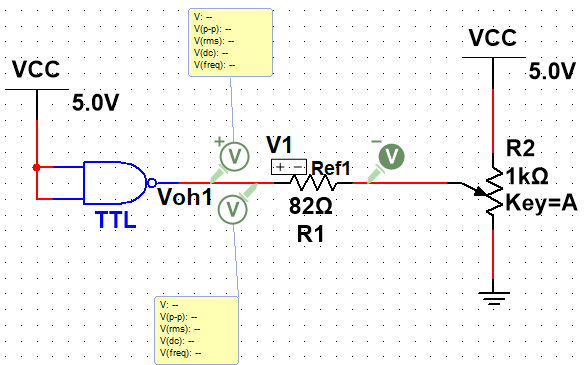
\includegraphics[width=0.5\textwidth]{part1c-ttl.png}	
    	\caption{The circuit using a TTL NAND gate.}
    	\label{fig:3-part1c-ttl}
\end{figure}

\paragraph{}The circuit given in figure \ref{fig:3-part1c-ttl} is implemented using a TTL NAND gate. The aim of this part is to find the maximum possible value of $I_{AB}$ when the output state of the gate is Logic-0. With the aid of the potentiometer $V_{output}$ is changed several times in order to see it's effects on $V_{AB}$. $I_{OH}$ values are calculated by using $V_{OH}/R$. All results of the mentioned part are given in Table \ref{part1c-ttl}.

%Table of part1c-ttl
\begin{table}[h]
\begin{tabular}{c|c|c|c|c|c|c|c|}
                & 1     & 2     & 3     & 4     & 5     & 6     & 7     \\ \hline
$V_{AB} (Volt)$ & -0.14 & -0.24 & -0.50 & -0.83 & -1.36 & -2.52 & -4.17 \\ \hline
$V_{OL} (Volt)$ & 0.14  & 0.19  & 0.24  & 0.28  & 0.32  & 0.42  & 0.57  \\ \hline
$I_{OL} (mA)$   & 1.70   & 2.90   & 6.00     & 10.00    & 16.50  & 30.70  & 50.80 
\end{tabular}
\centering
\caption{$V_{OL} - I_{OL}$ Characteristics of TTL}
\label{part1c-ttl}
\end{table}


 \begin{figure}[h]
    	\centering
    	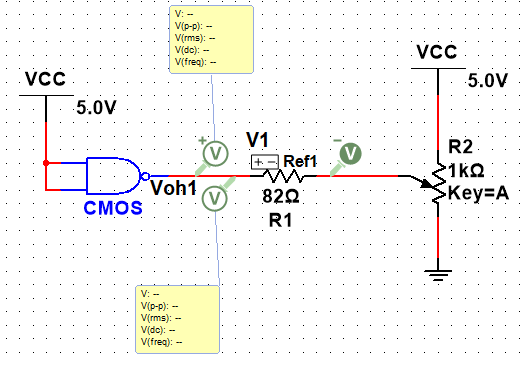
\includegraphics[width=0.5\textwidth]{part1c-cmos.png}	
    	\caption{The circuit using a CMOS NAND gate.}
    	\label{fig:3-part1c-cmos}
\end{figure}

\paragraph{}The circuit given in figure \ref{fig:3-part1c-cmos} is implemented using a CMOS NAND gate. The aim of this part is to find the maximum possible value of $I_{AB}$ when the output state of the gate is Logic-1. With the aid of the potentiometer $V_{output}$ is changed several times in order to see it's effects on $V_{AB}$. $I_{OH}$ values are calculated by using $V_{OH}/R$. All results are given in Table \ref{part1c-cmos}.

%Table of part1c-cmos
\begin{table}[h]
\begin{tabular}{c|c|c|c|c|c|c|c|}
                & 1 & 2     & 3     & 4     & 5     & 6     & 7     \\ \hline
$V_{AB} (Volt)$ & 0 & -0.35 & -0.51 & -0.55 & -0.56 & -0.57 & -0.58 \\ \hline
$V_{OL} (Volt)$ & 0 & 0.77  & 1.52  & 2.20  & 2.96  & 3.90  & 4.30  \\ \hline
$I_{OL} (mA)$   & 0 & 4.22  & 6.21  & 6.70  & 6.82  & 6.90  & 7.00 
\end{tabular}
\centering
\caption{$V_{OL} - I_{OL}$ Characteristics of CMOS}
\label{part1c-cmos}
\end{table}
\end{flushleft}


\newpage
 \begin{figure}[h]
    	\centering
    	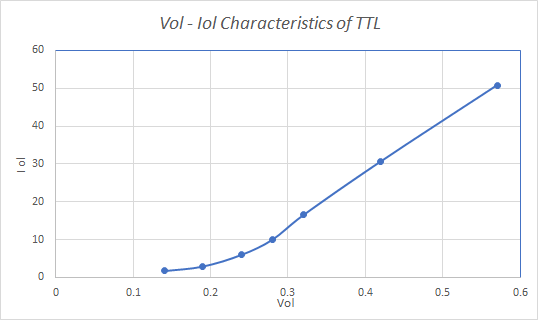
\includegraphics[width=0.7\textwidth]{charts/part1c-ttl-chart.png}	
    	\caption{$V_{OL} - I_{OL}$ Characteristics of TTL}
    	\label{graph:3-part1c-ttl}
\end{figure}

 \begin{figure}[h]
    	\centering
    	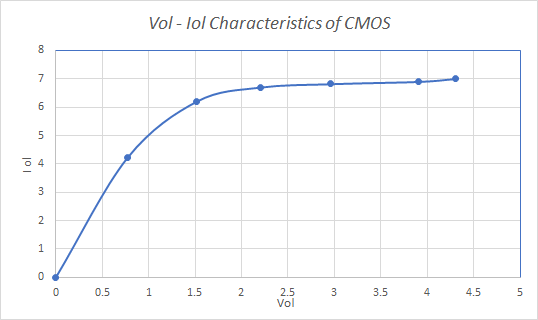
\includegraphics[width=0.7\textwidth]{charts/part1c-cmos-chart.png}	
    	\caption{$V_{OL} - I_{OL}$ Characteristics of CMOS}
    	\label{graph:3-part1c-cmoss}
\end{figure}


\begin{flushleft}
\paragraph{}

With this circuit, we were able to observe a wider voltage range with CMOS than TTL once again. This is once again due to the different reaction of both type of gates. It can be said that TTL is less reactive to the changes in current.
\end{flushleft}





\newpage
\begin{flushleft}
\subsubsection{Part 1.d}

 \begin{figure}[h]
    	\centering
    	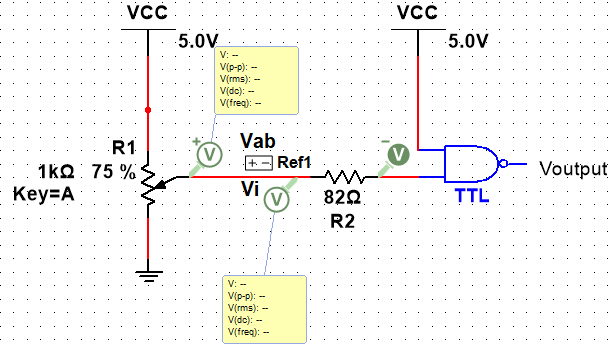
\includegraphics[width=0.5\textwidth]{part1d-ttl.png}
    	\caption{The circuit using a TTL NAND gate.}
    	\label{fig:4-part1d-ttl}
\end{figure}

\paragraph{}The circuit given in figure \ref{fig:4-part1d-ttl} is implemented using a TTL NAND gate. The aim of this part is to find $I_{input}$ values for different $V_{input}$. With the aid of the potentiometer $V_{i}$ is changed several times in order to see it's effects on $V_{AB}$. $I_{i}$ values are calculated by using $V_{AB}/R$. All results of the mentioned part are given in Table \ref{part1d-ttl}.

%Table of part1d-ttl
\begin{table}[h]
\begin{tabular}{c|c|c|c|c|c|c|c|}
               & 1     & 2      & 3    & 4 & 5    & 6    & 7    \\ \hline
$V_{AB} (mV)$  & -1.10 & -83.00 & -42  & 0 & 0    & 0    & 0    \\ \hline
$V_{i} (Volt)$ & 0     & 0.992  & 1.15 & 1.68 & 3.04 & 3.91 & 4.96 \\ \hline
$I_{i} (mA)$   & 1.35  & 1.01   & 0.51 & 0 & 0    & 0    & 0   
\end{tabular}
\centering
\caption{$V_{i} - I_{i}$ Characteristics of TTL}
\label{part1d-ttl}
\end{table}


 \begin{figure}[h]
    	\centering
    	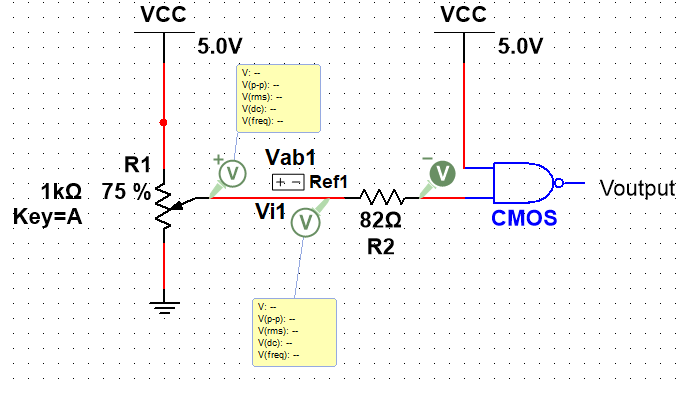
\includegraphics[width=0.5\textwidth]{part1d-cmos.png}
    	\caption{CMOS}
    	\label{fig:4-part1d-cmos}
\end{figure}

\paragraph{}The circuit given in figure \ref{fig:4-part1d-cmos} is implemented using a CMOS NAND gate. The aim of this part is to find $I_{input}$ values for different $V_{input}$. With the aid of the potentiometer $V_{i}$ is changed several times in order to see it's effects on $V_{AB}$. $I_{i}$ values are calculated by using $V_{AB}/R$. All results of the mentioned part are given in Table \ref{part1d-cmos}.

\begin{table}[h]
\begin{tabular}{c|c|c|c|c|c|c|c|}
               & 1 & 2    & 3    & 4    & 5    & 6    & 7    \\ \hline
$V_{AB} (V)$   & 0 & 0    & 0    & 0    & 0    & 0    & 0    \\ \hline
$V_{i} (Volt)$ & 0 & 0.65 & 1.18 & 2.16 & 3.60 & 4.40 & 4.97 \\ \hline
$I_{i} (mA)$   & 0 & 0    & 0    & 0    & 0    & 0    & 0   
\end{tabular}
\centering
\caption{$V_{i} - I_{i}$ Characteristics of CMOS}
\label{part1d-cmos}
\end{table}
\end{flushleft}


\newpage
 \begin{figure}[!h]
    	\centering
    	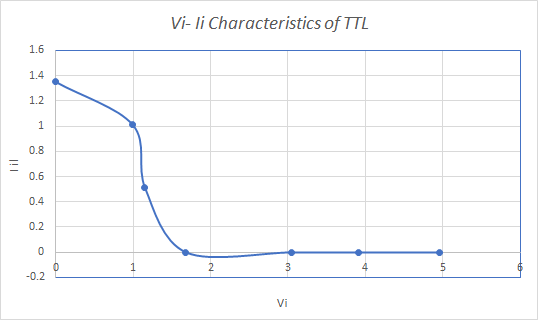
\includegraphics[width=0.7\textwidth]{charts/part1d-ttl-chart.png}	
    	\caption{$V_{i} - I_{i}$ Characteristics of TTL}
    	\label{graph:3-part1d-ttl}
\end{figure}

 \begin{figure}[!h]
    	\centering
    	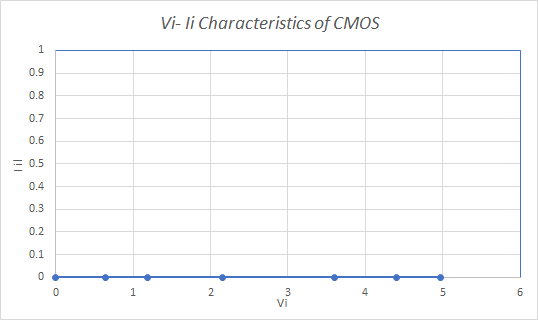
\includegraphics[width=0.7\textwidth]{charts/part1d-cmos-chart.png}
    	\caption{$V_{i} - I_{i}$ Characteristics of CMOS}
    	\label{graph:3-part1d-cmoss}
\end{figure}


\begin{flushleft}
\paragraph{}
In Figures \ref{graph:3-part1d-ttl} and \ref{graph:3-part1d-cmoss}, line graph of $V_i = f_4(I_i)$ is given. These lines do show how much a gate consumes when no output is connected. Figure \ref{graph:3-part1d-cmoss} shows one of the benefits of using CMOS gates which is not consuming any power when it is not needed, which will indicate that more CMOS gates can be connected sequentially than TTL gates can.
\end{flushleft}

\newpage
%neye yorumu yazalim ben tepeden asagi inerken fixleyeyim
% bi tek part2nin laflari kaldi ztn
% senin seyde yaziyordu frekansi hesaplamistik onu yazariz digeri de noise cikti duzgun hesaplayamadik diyip gecebiliriz ben yukardan fixleyerek geliyorum
%tamam..
\subsection{Part 2}

\paragraph{}
In the second part of the experiment, dynamic characteristics of TTL and CMOS NAND gates are observed.


 \begin{figure}[h]
    	\centering
    	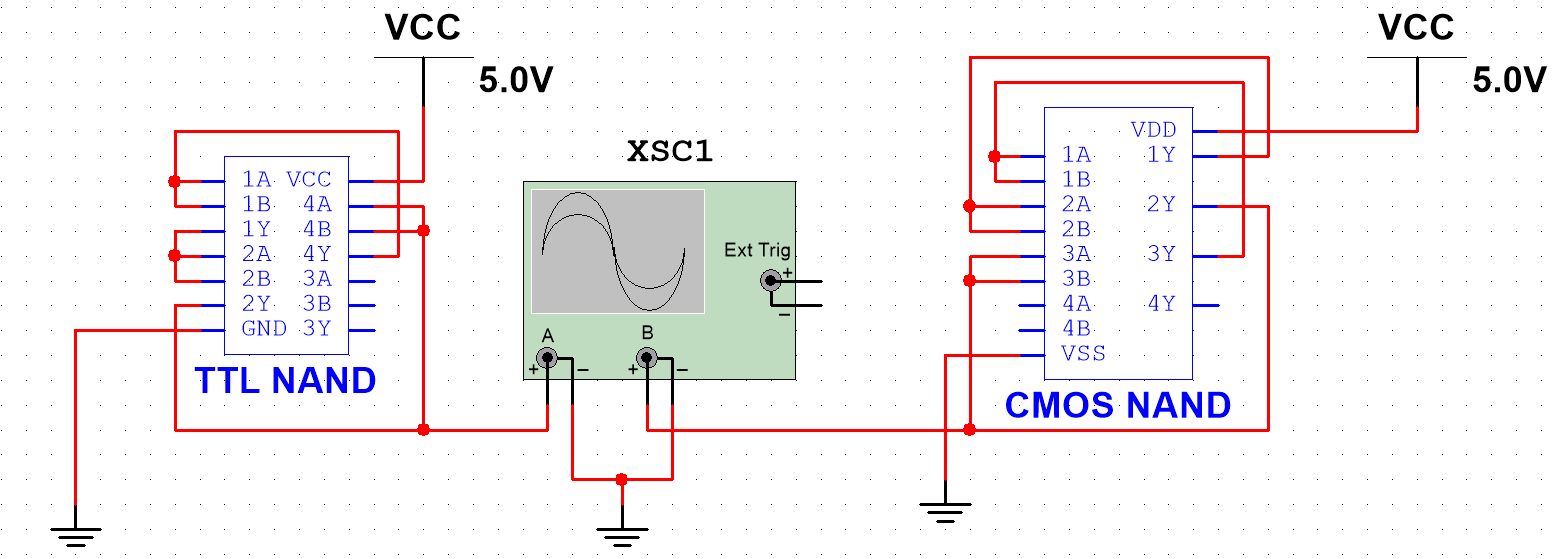
\includegraphics[width=1\textwidth]{part2.png}
    	\caption{PART 2}
    	\label{fig:5 part2}
\end{figure}

\begin{figure}[h]
    	\centering
    	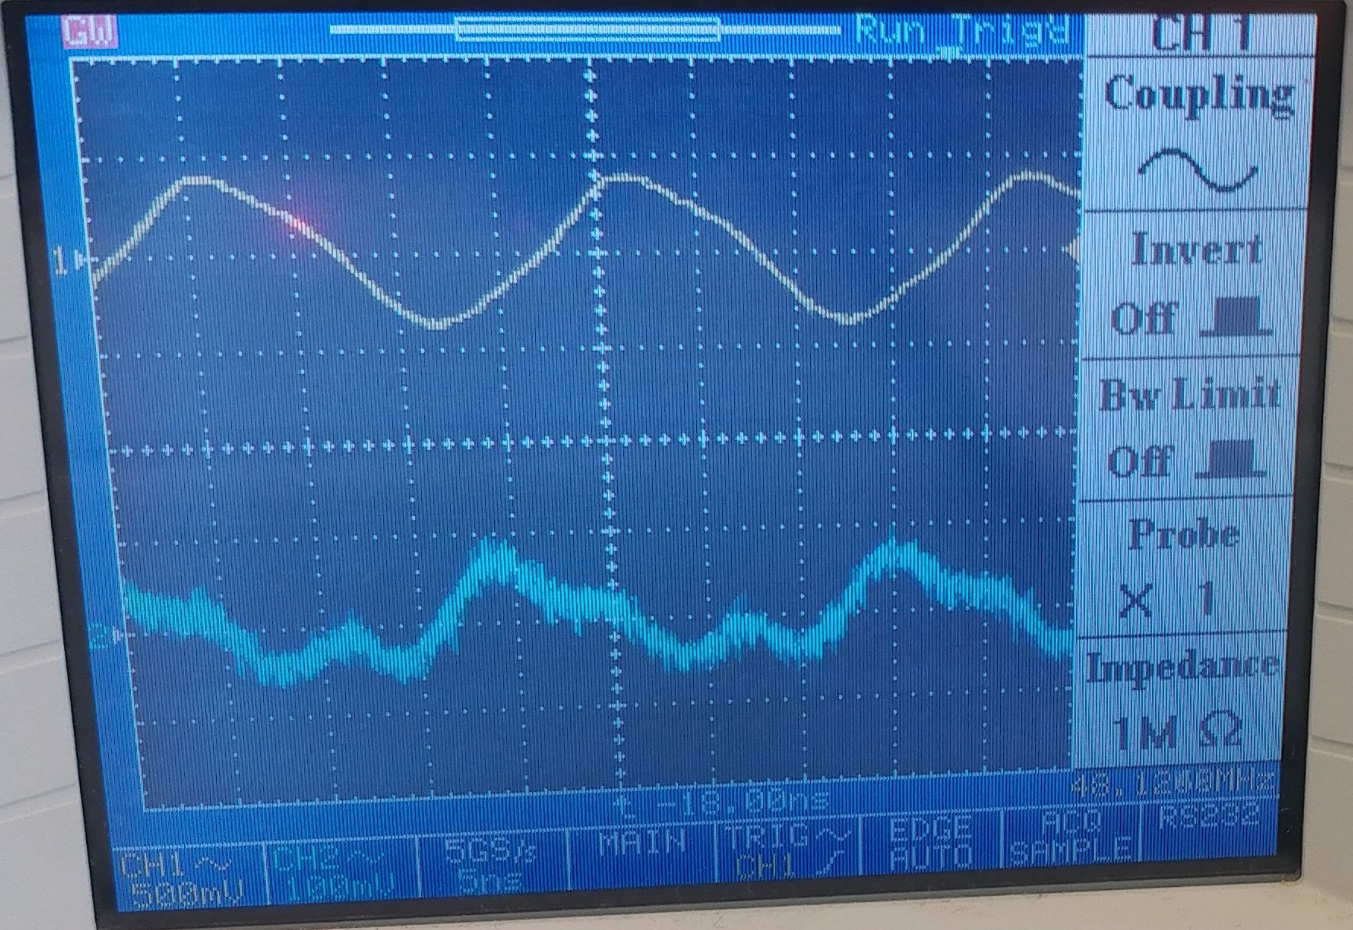
\includegraphics[width=0.5\textwidth]{Osiloskop.png}
    	\caption{PART 2}
    	\label{fig:6 part2}
\end{figure}


\begin{flushleft}
The circuit in \ref{fig:5 part2} was implemented using both CMOS and TTL gates. Both types of gates caused oscillation and that oscillation was monitored using the oscilloscope (as seen in \ref{fig:6 part2}). We also observed that there was some noise in the signal. But we were able to see a signal that was close to the result we were expecting for both types of gates. Frequency values for both circuits were close to 48 MHz, meaning the peroid was $2,08.10^{-9}$.
\end{flushleft}
% yolla yolla kaderim yolla
\newpage
\section{INTERPRETATION OF THE RESULTS}
Most of the experiment results were the way we expected them to be. But for some circuits, our results contradicted with the theoretically calculated values. For instance we were not able to get voltage values to zero for some circuits, which in theory should have been possible. We believe that this situation occurred because of the limitations with the equipment that has been used (maximum values for the potentiometers etc.).
\section{CONCLUSION}
While doing this experiment we were able to inspect the differences between TTL and CMOS behaviours in real life situations. And by doing so, we have acquired an improved vision for choosing the one that will be more suitable for our future designs. Also for the first time in an experiment, we had to finish the task as a 2 person group because of the fact that our friend Cihat unfortunately was eliminated from the laboratory. This truly affected our performance through the rest of the experiment resulting in us failing to complete one of the tasks.
\nocite{overleaf}
\nocite{reportGuide}
\newpage
\addcontentsline{toc}{section}{\numberline {}REFERENCES}

\bibliographystyle{unsrt}
\bibliography{reference}

\end{document}

